\section{Conclusion}

\pgfdeclareimage[width=1.0\paperwidth]{header-image}{header_images/post_fire}

\begin{frame}
    \frametitle{Humans reduce burnt area}
	\begin{itemize}
		\item Ignitions generally do not limit fire frequency
		\item Human-caused fire do result in burning, but normally areas that would have burnt anyway
		\item Vegetation models showing significant increases in fire frequency are doing something wrong somewhere
		\item Suppression efforts and land use have much bigger impact on fire
		\item from abstract
	\end{itemize}
\end{frame}

\begin{frame}
	\frametitle{Ignitions}
	\framesubtitle{Which is more important}
	%\node[anchor=south west,inner sep=0] (image) at (0,0) {
	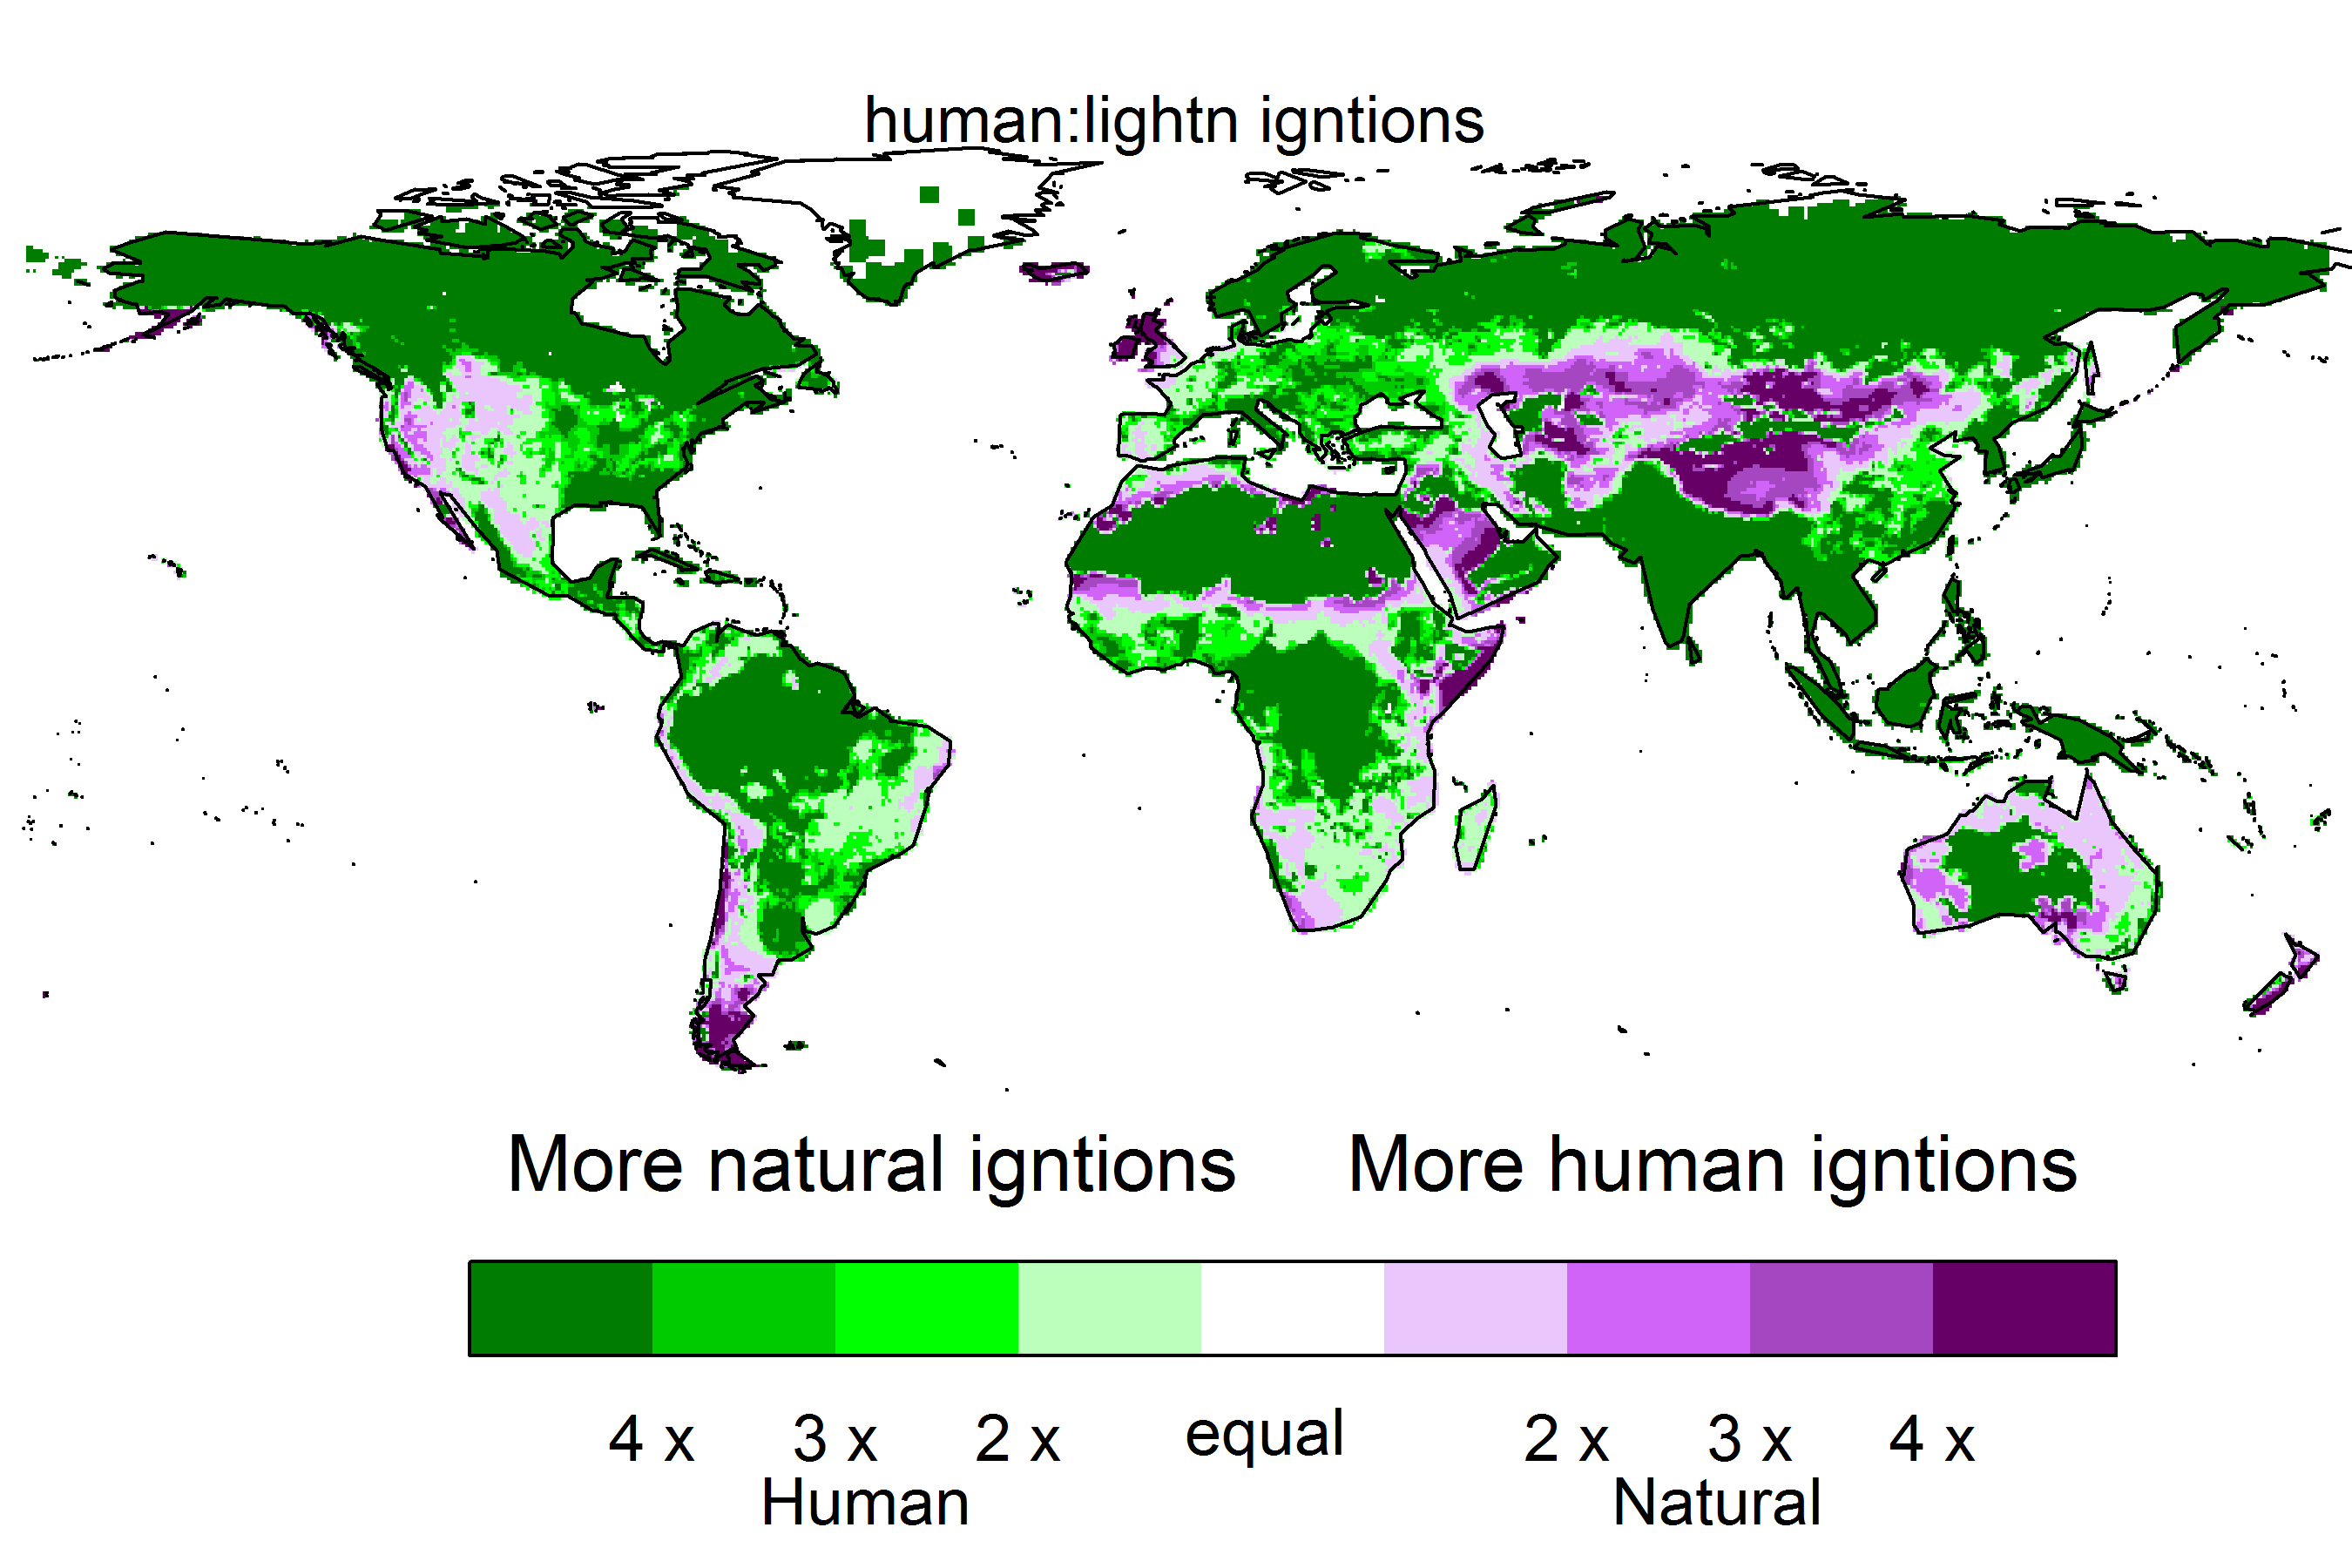
\includegraphics[width=11.0cm]{images/igntitions/IgntionInfosourceImportance}
	
\end{frame}

\begin{frame}
    \frametitle{Humans reduce burnt area}
	\large{But...}
	\begin{itemize}
		\item Human fires are a significant source, particularly pasture areas
		\item This would likely affect other aspects of fire regime (fire size, intensity etc)
		\item Other factors may influence fire frequency and fire controls on finer scales (e.g. topography)
	\end{itemize}
\end{frame}

\begin{frame}
    \frametitle{Acknowledgments}
    \framesubtitle{Questions..?}
\end{frame}
